\documentclass{beamer}
\mode<presentation>
\usepackage{amsmath,amssymb,mathtools}
\usepackage{textcomp}
\usepackage{gensymb}
\usepackage{adjustbox}
\usepackage{subcaption}
\usepackage{enumitem}
\usepackage{multicol}
\usepackage{listings}
\usepackage{url}
\usepackage{graphicx} % <-- needed for images
\def\UrlBreaks{\do\/\do-}

\usetheme{Boadilla}
\usecolortheme{lily}
\setbeamertemplate{footline}{
  \leavevmode%
  \hbox{%
  \begin{beamercolorbox}[wd=\paperwidth,ht=2ex,dp=1ex,right]{author in head/foot}%
    \insertframenumber{} / \inserttotalframenumber\hspace*{2ex}
  \end{beamercolorbox}}%
  \vskip0pt%
}
\setbeamertemplate{navigation symbols}{}

\lstset{
  frame=single,
  breaklines=true,
  columns=fullflexible,
  basicstyle=\ttfamily\tiny   % tiny font so code fits
}

\numberwithin{equation}{section}

% ---- your macros ----
\providecommand{\nCr}[2]{\,^{#1}C_{#2}}
\providecommand{\nPr}[2]{\,^{#1}P_{#2}}
\providecommand{\mbf}{\mathbf}
\providecommand{\pr}[1]{\ensuremath{\Pr\left(#1\right)}}
\providecommand{\qfunc}[1]{\ensuremath{Q\left(#1\right)}}
\providecommand{\sbrak}[1]{\ensuremath{{}\left[#1\right]}}
\providecommand{\lsbrak}[1]{\ensuremath{{}\left[#1\right.}}
\providecommand{\rsbrak}[1]{\ensuremath{\left.#1\right]}}
\providecommand{\brak}[1]{\ensuremath{\left(#1\right)}}
\providecommand{\lbrak}[1]{\ensuremath{\left(#1\right.}}
\providecommand{\rbrak}[1]{\ensuremath{\left.#1\right)}}
\providecommand{\cbrak}[1]{\ensuremath{\left\{#1\right\}}}
\providecommand{\lcbrak}[1]{\ensuremath{\left\{#1\right.}}
\providecommand{\rcbrak}[1]{\ensuremath{\left.#1\right\}}}
\theoremstyle{remark}
\newtheorem{rem}{Remark}
\newcommand{\sgn}{\mathop{\mathrm{sgn}}}
\providecommand{\abs}[1]{\left\vert#1\right\vert}
\providecommand{\res}[1]{\Res\displaylimits_{#1}}
\providecommand{\norm}[1]{\lVert#1\rVert}
\providecommand{\mtx}[1]{\mathbf{#1}}
\providecommand{\mean}[1]{E\left[ #1 \right]}
\providecommand{\fourier}{\overset{\mathcal{F}}{ \rightleftharpoons}}
\providecommand{\system}{\overset{\mathcal{H}}{ \longleftrightarrow}}
\providecommand{\dec}[2]{\ensuremath{\overset{#1}{\underset{#2}{\gtrless}}}}
\newcommand{\myvec}[1]{\ensuremath{\begin{pmatrix}#1\end{pmatrix}}}
\newcommand{\mydet}[1]{\ensuremath{\begin{vmatrix}#1\end{vmatrix}}}
\let\vec\mathbf
% ---------------------

\title{Matgeo Presentation - Problem 4.13.60}
\author{ee25btech11056 - Suraj.N}

\begin{document}

\begin{frame}
  \titlepage
\end{frame}

\begin{frame}{Problem Statement}

A line through $A(5,4)$ meets the lines 
$x+3y+2=0$, $2x+y+4=0$ and $x-y-5=0$ 
at $B,C,D$ respectively. If 
\[
\left(\frac{15}{AB}\right)^2 + \left(\frac{10}{AC}\right)^2 = \left(\frac{6}{AD}\right)^2,
\]
find the equation of the line.

\end{frame}

\begin{frame}{Data}

\begin{table}[h!]
  \centering
  \begin{tabular}{|c|c|}
\hline
\textbf{Name} & \textbf{Value} \\ \hline
$\vec{A}$ & $\myvec{2 & 1 \\0 & 3}$ \\ \hline
\end{tabular}

  \caption*{Table : Lines}
  \label{4.13.60}
\end{table}

\end{frame}

\begin{frame}{Solution}

Let the required line be
\begin{align}
\vec{x_4} &= \myvec{5\\4} + k\myvec{1\\m}
\end{align}

Hence the points $B,C,D$ can be written as
\begin{align}
\vec{B} &= \myvec{5\\4} + k_1\myvec{1\\m} = \myvec{5+k_1\\4+k_1m}  \\
\vec{C} &= \myvec{5\\4} + k_2\myvec{1\\m} = \myvec{5+k_2\\4+k_2m} \\
\vec{D} &= \myvec{5\\4} + k_3\myvec{1\\m} = \myvec{5+k_3\\4+k_3m} 
\end{align}

\end{frame}

\begin{frame}{Solution}

Find $k_1,k_2,k_3$\\
Since $\vec{B}$ lies on $\vec{x_1}$
\begin{align}
\myvec{\tfrac{1}{3} & 1}\vec{B} &= -\tfrac{2}{3}\\
\myvec{\tfrac{1}{3} & 1}\myvec{5+k_1\\4+k_1m} &= -\tfrac{2}{3}\\
\frac{17}{3}+\brak{m+\tfrac{1}{3}}k_1 &= -\tfrac{2}{3} \\
\brak{m+\tfrac{1}{3}}k_1 &= -\tfrac{19}{3} \\
k_1 &= \frac{-19}{3m+1}
\end{align}

\end{frame}

\begin{frame}{Solution}

Since $\vec{C}$ lies on $\vec{x_2}$
\begin{align}
\myvec{2 & 1}\vec{C} &= -4 \\
\myvec{2 & 1}\myvec{5+k_2\\4+k_2m} &= -4\\
(2+m)k_2+14 &= -4 \\
(2+m)k_2 &= -18 \\
k_2 &= \frac{-18}{m+2}
\end{align}

Since $\vec{D}$ lies on $\vec{x_3}$
\begin{align}
\myvec{-1 & 1}\vec{D} &= -5\\
\myvec{-1 & 1}\myvec{5+k_3\\4+k_3m} &= -5\\
(m-1)k_3-1 &= -5 \\
k_3 &= \frac{-4}{m-1}
\end{align}

\end{frame}

\begin{frame}{Solution}

Find distances
\begin{align}
  \norm{\vec{B}-\vec{A}} &= |k_1|\sqrt{1+m^2} \\
\norm{\vec{C}-\vec{A}} &= |k_2|\sqrt{1+m^2} \\
\norm{\vec{D}-\vec{A}} &= |k_3|\sqrt{1+m^2}
\end{align}

Use the given equation
\begin{align}
\left(\frac{15}{\norm{\vec{B}-\vec{A}}}\right)^2 
+ \left(\frac{10}{\norm{\vec{C}-\vec{A}}}\right)^2 
&= \left(\frac{6}{\norm{\vec{D}-\vec{A}}}\right)^2
\end{align}

Substitute distances:
\begin{align}
\frac{225}{k_1^2(1+m^2)} + \frac{100}{k_2^2(1+m^2)} 
&= \frac{36}{k_3^2(1+m^2)}
\end{align}

\end{frame}

\begin{frame}{Solution}

Multiply throughout by $(1+m^2)$:
\begin{align}
\frac{225}{k_1^2} + \frac{100}{k_2^2} &= \frac{36}{k_3^2}
\end{align}

Substitute values of $k_1,k_2,k_3$:
\begin{align}
\frac{225}{\brak{\tfrac{-19}{3m+1}}^2} + \frac{100}{\brak{\tfrac{-18}{m+2}}^2}
&= \frac{36}{\brak{\tfrac{-4}{m-1}}^2}
\end{align}

Simplify:
\begin{align}
\frac{225(3m+1)^2}{361} + \frac{100(m+2)^2}{324} &= \frac{9(m-1)^2}{4}\\
 \end{align}

\begin{align}
  429031m^2 + 1108138m -45869 &= 0
\end{align}

\end{frame}

\begin{frame}{Solution}

This gives a quadratic in $m$. Solving by using the quadratic formula, we get
\begin{align}
m &= 0.04075, \quad m = -2.62364
\end{align}

\textbf{Answer :}\\

Final equations of the line\\
For $m=0.04075$:

\begin{align}
  \vec{x_4} &= \myvec{5\\4} + k\myvec{1\\0.04075}
\end{align}

For $m=-2.62364:

\begin{align}
  \vec{x_4} &= \myvec{5\\4} + k\myvec{1\\-2.62364}
\end{align}

\end{frame}

\begin{frame}{Plot}

\begin{figure}[h!]
  \centering
  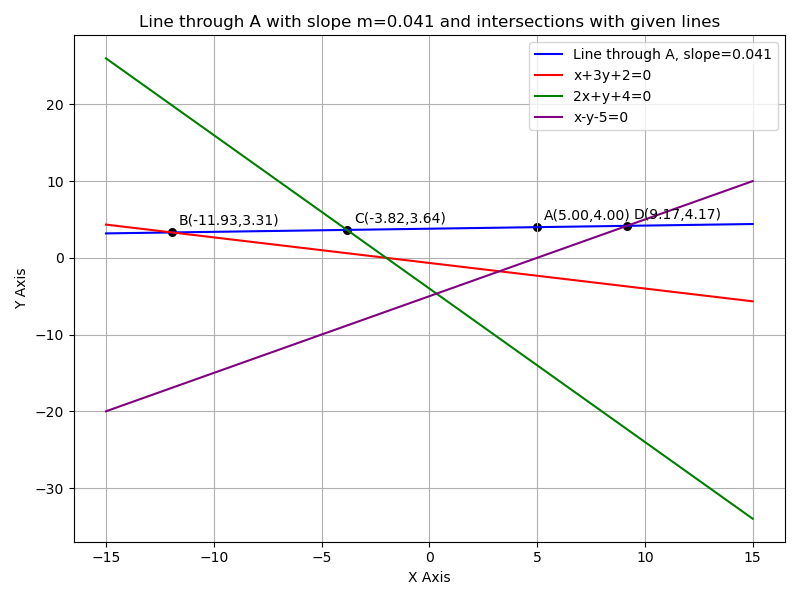
\includegraphics[width=0.8\columnwidth]{figs/lines_1.png} 
   \caption*{Fig : Lines 1}
  \label{Fig1}
\end{figure}

\end{frame}

\begin{frame}{Plot}

\begin{figure}[h!]
  \centering
  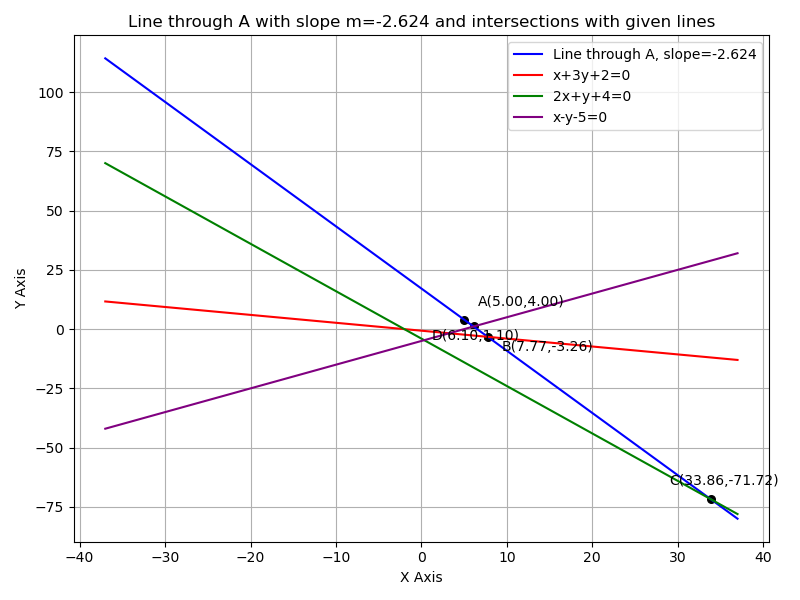
\includegraphics[width=0.8\columnwidth]{figs/lines_2.png} 
   \caption*{Fig : Lines 2}
  \label{Fig2}
\end{figure}

\end{frame}



\end{document}
